% Options for packages loaded elsewhere
\PassOptionsToPackage{unicode}{hyperref}
\PassOptionsToPackage{hyphens}{url}
\PassOptionsToPackage{dvipsnames,svgnames,x11names}{xcolor}
\documentclass[
  11pt,
]{article}
\usepackage{xcolor}
\usepackage[margin=0.85in]{geometry}
\usepackage{amsmath,amssymb}
\setcounter{secnumdepth}{-\maxdimen} % remove section numbering
\usepackage{iftex}
\ifPDFTeX
  \usepackage[T1]{fontenc}
  \usepackage[utf8]{inputenc}
  \usepackage{textcomp} % provide euro and other symbols
\else % if luatex or xetex
  \usepackage{unicode-math} % this also loads fontspec
  \defaultfontfeatures{Scale=MatchLowercase}
  \defaultfontfeatures[\rmfamily]{Ligatures=TeX,Scale=1}
\fi
\usepackage{lmodern}
\ifPDFTeX\else
  % xetex/luatex font selection
\fi
% Use upquote if available, for straight quotes in verbatim environments
\IfFileExists{upquote.sty}{\usepackage{upquote}}{}
\IfFileExists{microtype.sty}{% use microtype if available
  \usepackage[]{microtype}
  \UseMicrotypeSet[protrusion]{basicmath} % disable protrusion for tt fonts
}{}
\makeatletter
\@ifundefined{KOMAClassName}{% if non-KOMA class
  \IfFileExists{parskip.sty}{%
    \usepackage{parskip}
  }{% else
    \setlength{\parindent}{0pt}
    \setlength{\parskip}{6pt plus 2pt minus 1pt}}
}{% if KOMA class
  \KOMAoptions{parskip=half}}
\makeatother
\usepackage{color}
\usepackage{fancyvrb}
\newcommand{\VerbBar}{|}
\newcommand{\VERB}{\Verb[commandchars=\\\{\}]}
\DefineVerbatimEnvironment{Highlighting}{Verbatim}{commandchars=\\\{\}}
% Add ',fontsize=\small' for more characters per line
\newenvironment{Shaded}{}{}
\newcommand{\AlertTok}[1]{\textcolor[rgb]{1.00,0.00,0.00}{\textbf{#1}}}
\newcommand{\AnnotationTok}[1]{\textcolor[rgb]{0.38,0.63,0.69}{\textbf{\textit{#1}}}}
\newcommand{\AttributeTok}[1]{\textcolor[rgb]{0.49,0.56,0.16}{#1}}
\newcommand{\BaseNTok}[1]{\textcolor[rgb]{0.25,0.63,0.44}{#1}}
\newcommand{\BuiltInTok}[1]{\textcolor[rgb]{0.00,0.50,0.00}{#1}}
\newcommand{\CharTok}[1]{\textcolor[rgb]{0.25,0.44,0.63}{#1}}
\newcommand{\CommentTok}[1]{\textcolor[rgb]{0.38,0.63,0.69}{\textit{#1}}}
\newcommand{\CommentVarTok}[1]{\textcolor[rgb]{0.38,0.63,0.69}{\textbf{\textit{#1}}}}
\newcommand{\ConstantTok}[1]{\textcolor[rgb]{0.53,0.00,0.00}{#1}}
\newcommand{\ControlFlowTok}[1]{\textcolor[rgb]{0.00,0.44,0.13}{\textbf{#1}}}
\newcommand{\DataTypeTok}[1]{\textcolor[rgb]{0.56,0.13,0.00}{#1}}
\newcommand{\DecValTok}[1]{\textcolor[rgb]{0.25,0.63,0.44}{#1}}
\newcommand{\DocumentationTok}[1]{\textcolor[rgb]{0.73,0.13,0.13}{\textit{#1}}}
\newcommand{\ErrorTok}[1]{\textcolor[rgb]{1.00,0.00,0.00}{\textbf{#1}}}
\newcommand{\ExtensionTok}[1]{#1}
\newcommand{\FloatTok}[1]{\textcolor[rgb]{0.25,0.63,0.44}{#1}}
\newcommand{\FunctionTok}[1]{\textcolor[rgb]{0.02,0.16,0.49}{#1}}
\newcommand{\ImportTok}[1]{\textcolor[rgb]{0.00,0.50,0.00}{\textbf{#1}}}
\newcommand{\InformationTok}[1]{\textcolor[rgb]{0.38,0.63,0.69}{\textbf{\textit{#1}}}}
\newcommand{\KeywordTok}[1]{\textcolor[rgb]{0.00,0.44,0.13}{\textbf{#1}}}
\newcommand{\NormalTok}[1]{#1}
\newcommand{\OperatorTok}[1]{\textcolor[rgb]{0.40,0.40,0.40}{#1}}
\newcommand{\OtherTok}[1]{\textcolor[rgb]{0.00,0.44,0.13}{#1}}
\newcommand{\PreprocessorTok}[1]{\textcolor[rgb]{0.74,0.48,0.00}{#1}}
\newcommand{\RegionMarkerTok}[1]{#1}
\newcommand{\SpecialCharTok}[1]{\textcolor[rgb]{0.25,0.44,0.63}{#1}}
\newcommand{\SpecialStringTok}[1]{\textcolor[rgb]{0.73,0.40,0.53}{#1}}
\newcommand{\StringTok}[1]{\textcolor[rgb]{0.25,0.44,0.63}{#1}}
\newcommand{\VariableTok}[1]{\textcolor[rgb]{0.10,0.09,0.49}{#1}}
\newcommand{\VerbatimStringTok}[1]{\textcolor[rgb]{0.25,0.44,0.63}{#1}}
\newcommand{\WarningTok}[1]{\textcolor[rgb]{0.38,0.63,0.69}{\textbf{\textit{#1}}}}
\usepackage{graphicx}
\makeatletter
\newsavebox\pandoc@box
\newcommand*\pandocbounded[1]{% scales image to fit in text height/width
  \sbox\pandoc@box{#1}%
  \Gscale@div\@tempa{\textheight}{\dimexpr\ht\pandoc@box+\dp\pandoc@box\relax}%
  \Gscale@div\@tempb{\linewidth}{\wd\pandoc@box}%
  \ifdim\@tempb\p@<\@tempa\p@\let\@tempa\@tempb\fi% select the smaller of both
  \ifdim\@tempa\p@<\p@\scalebox{\@tempa}{\usebox\pandoc@box}%
  \else\usebox{\pandoc@box}%
  \fi%
}
% Set default figure placement to htbp
\def\fps@figure{htbp}
\makeatother
\setlength{\emergencystretch}{3em} % prevent overfull lines
\providecommand{\tightlist}{%
  \setlength{\itemsep}{0pt}\setlength{\parskip}{0pt}}
\usepackage{amsmath,amssymb}
\usepackage{float}
\usepackage{microtype}
\usepackage{fvextra}
\fvset{breaklines=true}
\usepackage{setspace}
\usepackage{lineno}
\usepackage{etoolbox}
\usepackage{needspace}
\usepackage{xurl}
\AtBeginEnvironment{longtable}{\singlespacing\small}
\AtBeginEnvironment{verbatim}{\singlespacing\small}
\setlength{\emergencystretch}{3em}
\floatplacement{figure}{H}
\DeclareUnicodeCharacter{2212}{\ensuremath{-}}
\DeclareUnicodeCharacter{2264}{\ensuremath{\leq}}
\DeclareUnicodeCharacter{2265}{\ensuremath{\geq}}
\DeclareUnicodeCharacter{2260}{\ensuremath{\ne}}
\DeclareUnicodeCharacter{2208}{\ensuremath{\in}}
\DeclareUnicodeCharacter{221E}{\ensuremath{\infty}}
\DeclareUnicodeCharacter{03B4}{\ensuremath{\delta}}
\DeclareUnicodeCharacter{03BB}{\ensuremath{\lambda}}
\DeclareUnicodeCharacter{03C4}{\ensuremath{\tau}}
\DeclareUnicodeCharacter{03BA}{\ensuremath{\kappa}}
\DeclareUnicodeCharacter{03B3}{\ensuremath{\gamma}}
\DeclareUnicodeCharacter{03B5}{\ensuremath{\varepsilon}}
\DeclareUnicodeCharacter{03C6}{\ensuremath{\phi}}
\DeclareUnicodeCharacter{2124}{\ensuremath{\mathbb Z}}
\DeclareUnicodeCharacter{1D63}{\ensuremath{{}_r}}
\DeclareUnicodeCharacter{2080}{\ensuremath{{}_0}}
\DeclareUnicodeCharacter{208A}{\ensuremath{{}_+}}
\DeclareUnicodeCharacter{208B}{\ensuremath{{}_-}}
\DeclareUnicodeCharacter{207B}{\ensuremath{{}^{-}}}
\DeclareUnicodeCharacter{00B9}{\ensuremath{{}^{1}}}
\DeclareUnicodeCharacter{00B2}{\ensuremath{{}^{2}}}
\DeclareUnicodeCharacter{2074}{\ensuremath{{}^{4}}}
\DeclareUnicodeCharacter{2075}{\ensuremath{{}^{5}}}
\DeclareUnicodeCharacter{2076}{\ensuremath{{}^{6}}}
\DeclareUnicodeCharacter{2192}{\ensuremath{\rightarrow}}
\DeclareUnicodeCharacter{0108}{\ensuremath{\widehat C}}
\DeclareUnicodeCharacter{00C2}{\ensuremath{\widehat A}}

\AtBeginDocument{\setstretch{1.12}}
\usepackage{bookmark}
\IfFileExists{xurl.sty}{\usepackage{xurl}}{} % add URL line breaks if available
\urlstyle{same}
% fallback for those not using the hyperref driver hyperxmp:
\makeatletter
\@ifundefined{xmpquote}{\newcommand{\xmpquote}[1]{#1}}{}
\makeatother
\hypersetup{
  colorlinks=true,
  linkcolor={Maroon},
  filecolor={Maroon},
  citecolor={Blue},
  urlcolor={blue},
  pdfcreator={LaTeX via pandoc}}

\author{}
\date{}

\begin{document}

\section{Additional file 6: Reproducibility
details}\label{additional-file-6-reproducibility-details}

These records describe retained computational evidence. The complete
inputs are provided through the v0.2.0 study archive identified in the
main article. Full stored-map replay is distinct from verification of
exported scalar results. Provider output terms and modification notices
accompany the archive.

The within-site analyses and their numerical record are archived in the
existing AlphaGenome reproduction package {[}1{]}. Its source code,
curation records and supplementary tables give the complete empirical
methods. An extraction manifest records selected machine-artifact values
and hashes; extraction does not constitute independent regeneration of
all earlier analyses. A separate targeted cache check reproduces the
three reported AVI stratum counts and mean statistics and records their
tie frequencies; it does not rerun their permutation tests. The schema
probe and mathematical-example verifier accompany the present analysis.
The verifier checks interval translation, scale normalization, paired
diagram-alignment bounds, nonmonotonicity under vertex deletion, the
distinction between bottleneck and Betti-curve distances, the failure of
treating an arbitrary contact transform as a metric, tie-aware
conditional nulls and rank invariance. No result from these finite
examples is labeled a genomic observation.

The completed spatial reproduction bundle includes all raw per-call
reference/alternate maps, assembled site arrays, coordinates, track
metadata, input hashes, the locally frozen protocol, exact-matching
settings, full diagrams, all sixteen conditional tests, numerical
diagnostics and acquisition audits. The AlphaGenome client was version
0.9.0; its non-generated Python source matched the recorded vendored
commit. ALL\_FOLDS is a model alias; an immutable server weight revision
was not exposed. The strengthened mathematical verifier passed eight
check groups, including 100 randomized quotient comparisons. Independent
inference checks include exhaustive finite-label distributions. These
finite checks do not by themselves constitute a Lean formalization, a
clean-environment regeneration of the retained audit, or biological
validation.

The anchor extension additionally contains the frozen replication cohort
and protocol, all 84 sites' raw predictions, native diagrams, 252
endpoint comparisons, 21 direct midpoint checks, scalar reconstruction
baselines, known-answer controls and independent derived-count checks.
Exact rational finite checks exercise the local slope and
endpoint-envelope arguments; independent Hera checks include turning and
flat controls. The prospective engine retains failures and source
hashes, and did not exclude any planned site. The numerical comparison
tolerances and their limits accompany the outputs. Additional file 2
supplies the full proofs and counterexamples, and the integration map
supplied with the review package records how this replacement
incorporates the earlier contribution.

A subsequent validation pass regenerated all 204 spatial sites from
cached maps in a fresh environment, including full diagrams, endpoint
distances and the fixed midpoint checks. All 6,324 per-site comparisons
passed the declared tolerances; 18 centered-distance vectors differed
only at floating-point rounding scale. All sixteen conditional tests
were independently recertified from the new outputs. The six retained
historical output files regenerated byte-for-byte using their retained
original random seeds. This checks execution reproducibility, not Monte
Carlo precision. Linkage to each output is recorded in the validation
report. The portable reproduction package pins its dependencies, inputs
and expected outputs and preserves the failed setup and postprocessing
attempts alongside their repairs. This reproduction checks computations
on the retained inputs; it does not establish model accuracy or
immutable server weights.

The cross-track extension retains its pre-acquisition protocol, all 252
two-track calls, the independently checked GM12878 drift control, the
native-prediction lock, per-site diagrams and centered validations, and
a full reference-engine replay using the original persistent-homology
implementation. A separate computational audit recomputed Hausdorff
witnesses by brute force and reconstructed rankings and rational
selected-allele credits from per-site files. The only execution
correction was an initial import failure in the acquisition environment;
the unchanged analysis ran in the existing fresh validation environment.
Failed import logs and actual dependency versions are preserved. The
portability validation report supplied with the review package
distinguishes the new checks from the preceding full harness and its
remaining human and provenance requirements.

\subsection{Targeted Julia persistence
check}\label{targeted-julia-persistence-check}

A subsequent targeted check used Ripserer 0.17.0 {[}2{]} under Julia
1.13.0 to reconstruct full H1 diagrams from saved maps. The sample
combined the previously frozen smallest-hash site in each of the seven
replication genes (indices 7, 21, 34, 44, 59, 70 and 75) with every site
containing a known IMR-90 nonsaturation exception (48, 51 and 59). The
union comprised nine sites on both GM12878 and IMR-90 tracks. Reference
and all three alternate maps gave 72 diagrams, 18 site-track records and
54 reference-alternate pairs. Selection preceded the Julia outcomes but
deliberately included known exceptions; this was targeted computational
validation, not a new prospective biological sample.

Each map retained all 512 bins and 130,816 unordered edges. The Julia
runner received raw maps and identifiers, not expected diagrams, and
independently reconstructed the complete weighted flag filtration over
\(\mathbb{F}_2\). It reproduced the original offset and effective
float32 edge inputs, used an infinite filtration threshold with no
positive-lifetime censoring, and restored the original float64 offset
after converting output coordinates to float64. Comparison required
exact equality of the complete interval multisets, preserving repeated
intervals rather than deduplicating them. All 72 diagrams, comprising
847,288 intervals, matched exactly. Effective input hashes, offsets and
independently computed map means also agreed.

Before the genomic calculation, 22 small-graph controls matched a
separate explicit boundary-matrix reduction over \(\mathbb{F}_2\): ten
named controls with hand-derived answers and twelve fixed-seed random
graphs. Controls covered negative and zero births, ties, repeated
intervals, nonmetric weights, an inactive edge, float32 near-tie
collapse, translation and ignored matrix diagonals. Four deliberately
corrupted comparisons were rejected: a missing duplicate interval, a
changed endpoint, an unrestored offset and a corrupted input hash.

Downstream reconstruction from the Julia diagrams matched all 108
native/centered bottleneck distances and all 54 shifted Hausdorff
witnesses exactly; all 2,565 recorded checks passed. The witness
calculation used a separate blockwise all-pairs implementation with
diagonal alternatives. Top sets and fractional credits matched at
tolerances 0, \(10^{-6}\) and \(10^{-5}\); stored GM12878 bound
predictions were checked at \(10^{-6}\) and IMR-90 predictions at all
three tolerances. All three known IMR-90 exceptions remained: site
48/ALT index 2, site 51/ALT index 1 and site 59/ALT index 0. Their
absolute saturation residuals were respectively 0.001204502435174145,
0.002583775381601489 and 0.00014162732143801343. Neither the full-cohort
results nor the scientific conclusions changed.

Ripserer is a separate implementation in the Ripser algorithm family.
Downstream bottleneck matching retained the shared GUDHI/Hera solver at
approximation parameter zero. Exact agreement concerns the effective
float32 filtration inputs and restored coordinates; it does not certify
unrounded real-valued maps, the complete numerical error allowance, or
every site in the study. The check does not establish independent-model
transfer, biological validity or clinical superiority. It supplies no
Lean formalization and does not repeat the separate exact-rational
conditional label tests.

The protocol, Julia runner, genomic inputs and primary comparator
remained unchanged during genomic execution. After the initial source
freeze, three receipt identity/hash assertions and a corrected
explanatory docstring were added to the control comparator; control
inputs and expected results were unchanged, and the stricter comparison
passed. The original files, amendment and execution receipts are
retained. Pinned Julia and Python environments, raw selected inputs,
computed diagrams, comparison code, outputs and logs are supplied in the
separate
\href{https://github.com/patrickiben/contact-map-anchor-audit/releases/download/v0.2.3/JULIA_PERSISTENCE_VALIDATION_2026-10-28.zip}{Julia
validation capsule}, 88,338,909 bytes, SHA-256:

\begin{Shaded}
\begin{Highlighting}[]
\NormalTok{e795faca8ba6217ccc4a2876f8a2613095f8dc8c175c86d41909092a7a36df54}
\end{Highlighting}
\end{Shaded}

The capsule was published as an addendum validating manuscript v0.2.3;
its preserved report describes that earlier manuscript state. It is
separate from the v0.2.0 full-study archive. Portable workspace
preparation and relocated controls were checked; those packaging checks
are not a second complete genomic replay. The source and result records
are also available in the
\href{https://github.com/patrickiben/contact-map-anchor-audit/tree/cd7b1352885f73dca0e1b1477c96d1db39a97382/research/julia_validation}{versioned
Julia validation directory}. These checks supplement the earlier
validation harness and author review; they are not external human peer
review.

\subsection{Cited resources}\label{cited-resources}

\begin{enumerate}
\def\labelenumi{\arabic{enumi}.}
\tightlist
\item
  Iben P. Reproducibility package for ``What do within-site comparisons
  of AlphaGenome Atlas predictions measure? An audit at ClinVar sites in
  11 genes''. Zenodo, version 1.0, 2026.
  \href{https://doi.org/10.5281/zenodo.23537469}{doi:10.5281/zenodo.23537469}.
\item
  Čufar M. Ripserer.jl: flexible and efficient persistent homology
  computation in Julia. \emph{Journal of Open Source Software}.
  2020;5(54):2614.
  \href{https://doi.org/10.21105/joss.02614}{doi:10.21105/joss.02614}.
\end{enumerate}

\subsection{Fixed illustrative site}\label{fixed-illustrative-site}

\par\noindent\begin{minipage}{\linewidth}

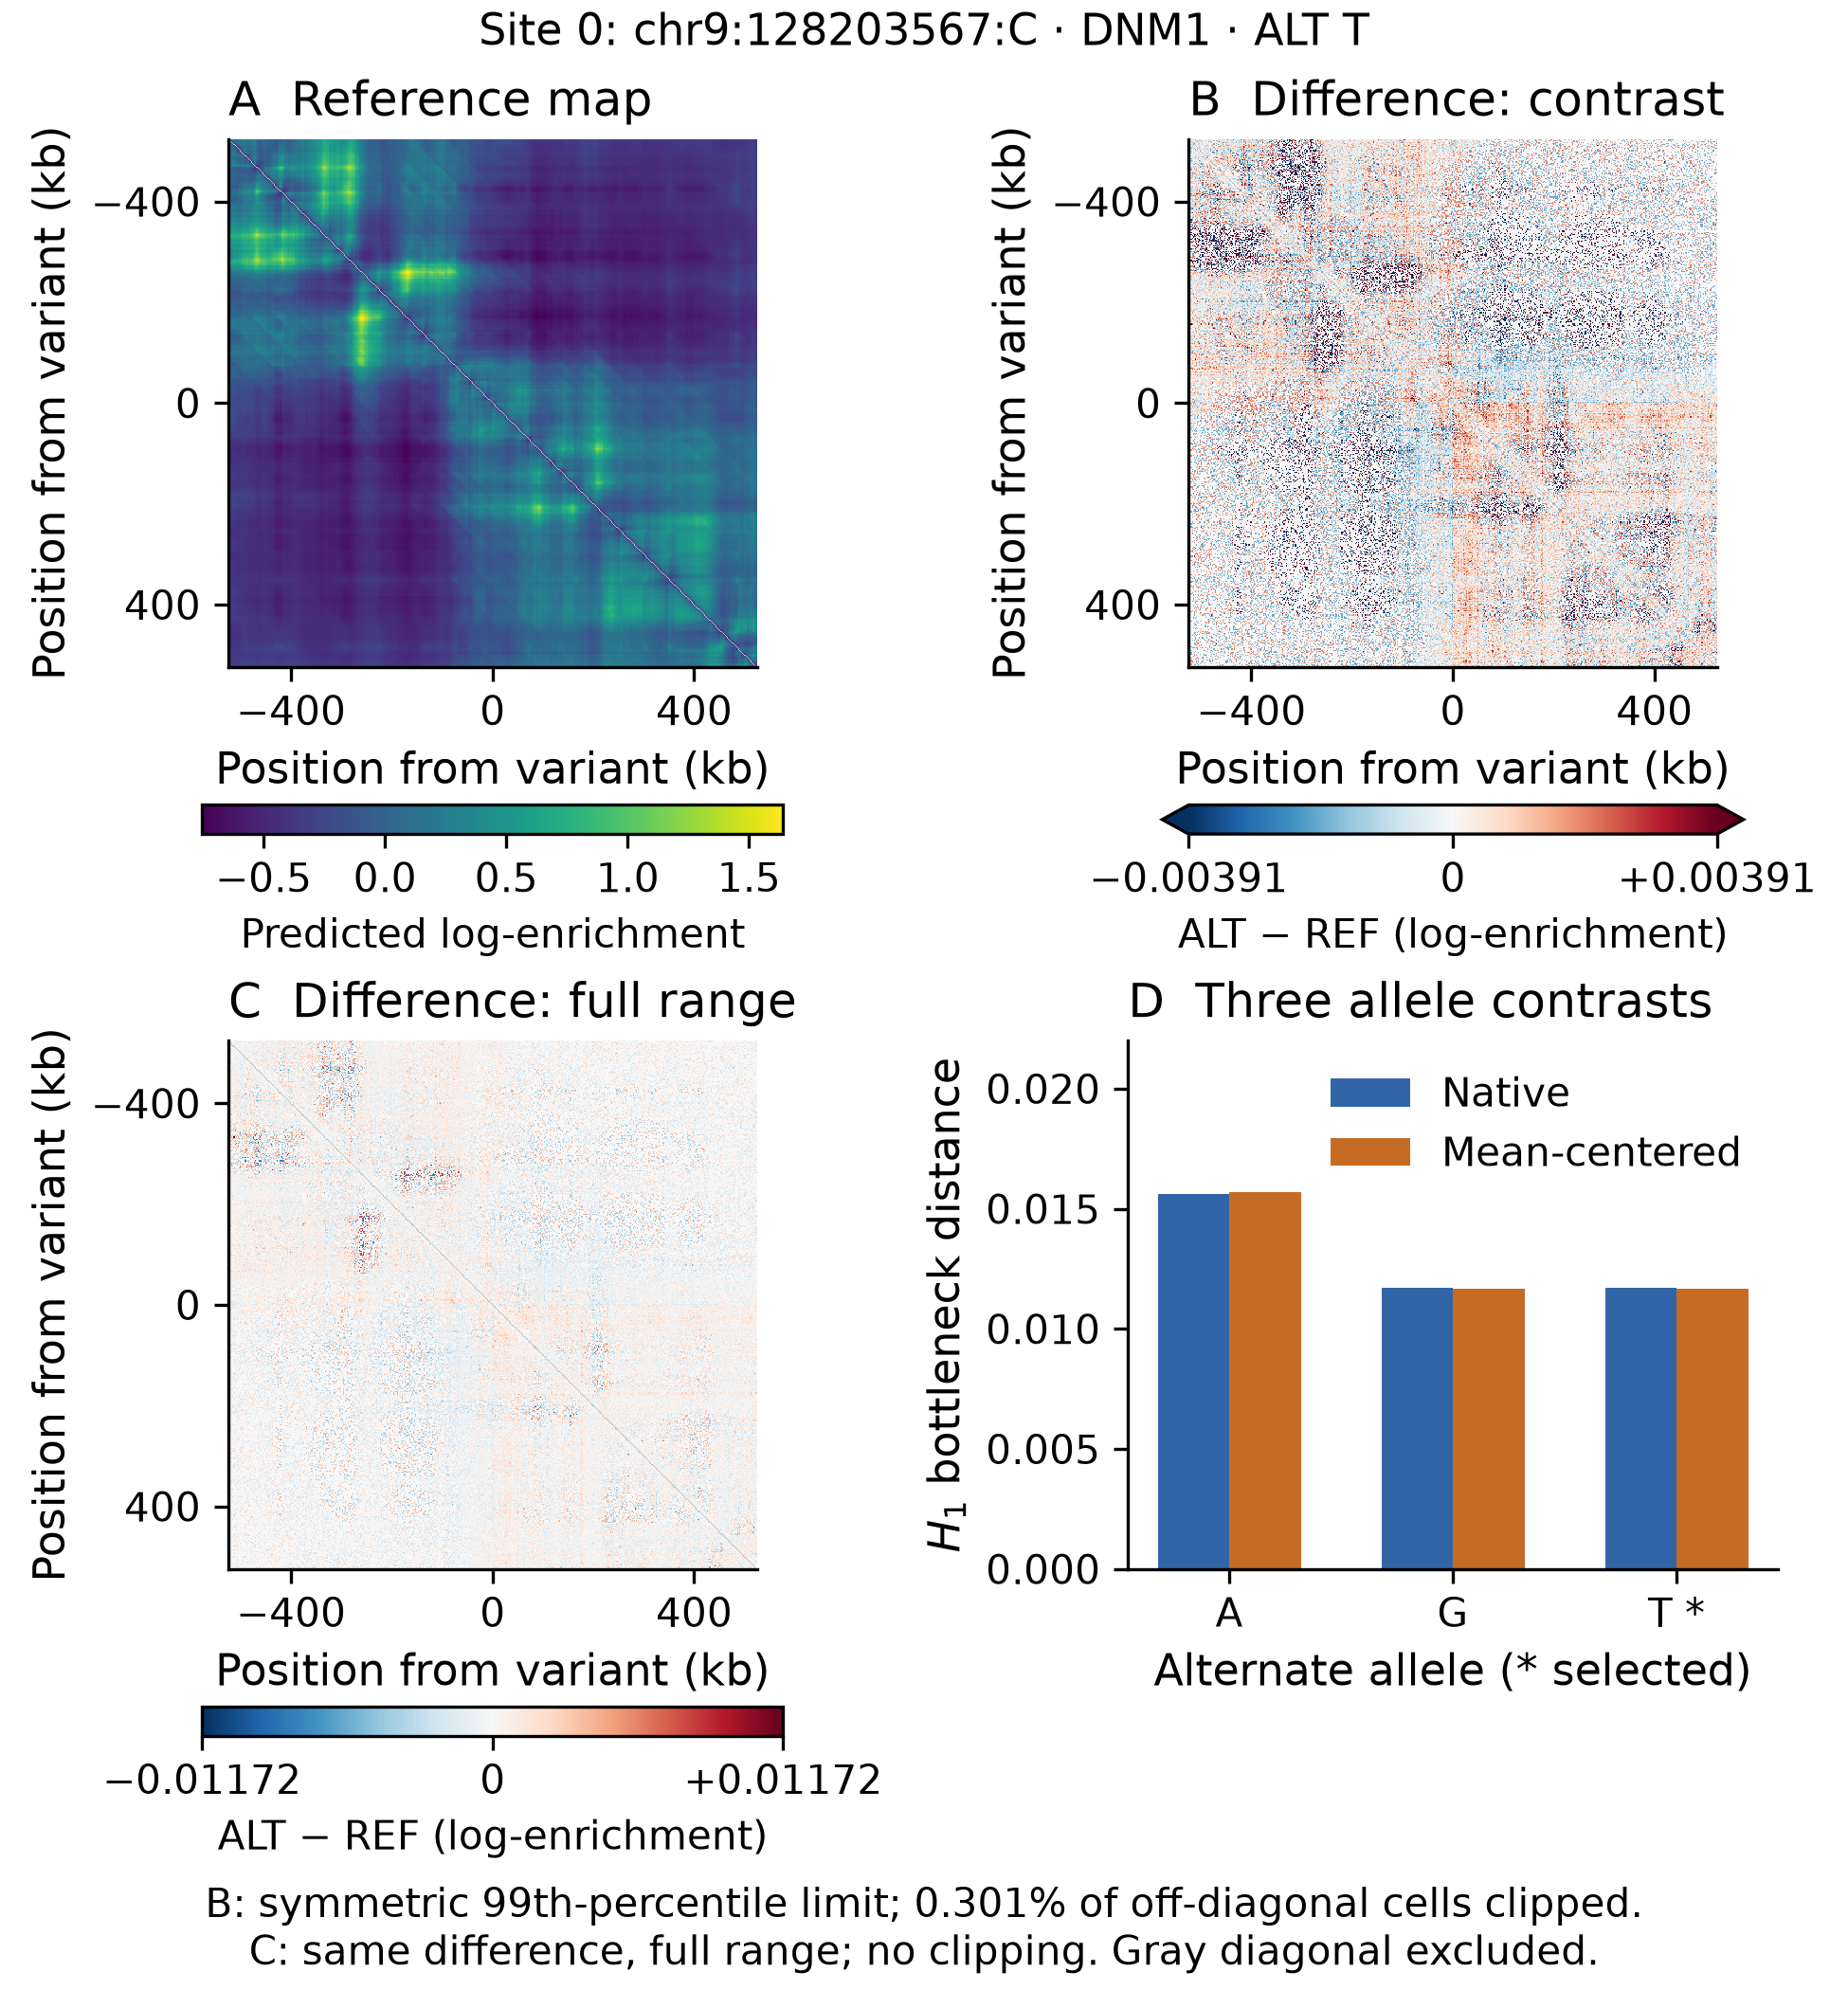
\includegraphics[width=6.5in,height=\textheight,keepaspectratio,alt={Fixed first genomic site with contrast and full-range difference views}]{figures/figure_s6_first_genomic_site.png}

\textbf{Figure S6.1.} Fixed input-order site zero (chr9:128203567:C;
DNM1; GM12878), not selected by effect size. \textbf{A}, reference
predicted log-enrichment. \textbf{B}, selected-alternate T minus
reference, with linear limits ±0.00390625 (99th percentile of absolute
off-diagonal differences): 788/261632 cells (0.301\%) color-clipped.
\textbf{C}, identical differences at full linear range ±0.01171875,
without clipping. Both scales are zero-centered in log-enrichment
difference units. \textbf{D}, native and mean-centered H1 bottleneck
distances for three alternate alleles; the asterisk marks the
ClinVar-selected allele. Gray diagonals are excluded. No physical loop
validation is implied. AlphaGenome-derived material remains subject to
provider Output Terms identified in the main article.

\end{minipage}\par

\end{document}
